\chapter{Ergebnisse und Analyse}

Dieses Kapitel bietet einen umfassenden Überblick über die Funktionalität und die Benutzerfreundlichkeit der E-Commerce-Webanwendung, die anhand einer Reihe detaillierter Screenshots und Analysen vorgestellt wird. Es werden die wichtigsten Funktionen der Anwendung untersucht, beginnend mit dem Anmeldeprozess, der einen sicheren Benutzerzugang gewährleistet, gefolgt von den Produktsuchfunktionen, die es dem Benutzer ermöglichen, Artikel nach Schlüsselwort oder Kategorie zu finden. Der Prozess des Hinzufügens von Produkten in den Einkaufswagen, das Fortschreiten zur Kasse und das Abschließen von Zahlungen wird veranschaulicht, um die nahtlose Integration dieser wesentlichen E-Commerce-Funktionen zu demonstrieren. Darüber hinaus wird in diesem Kapitel die Funktion „Bestellhistorie“ erläutert, mit der Benutzer frühere Einkäufe überprüfen können. Auch die Seiten mit eingeschränktem Zugriff, die nur angemeldeten Benutzern zur Verfügung stehen, werden besprochen, wobei die verbesserte Benutzerfreundlichkeit und die implementierten Sicherheitsmaßnahmen hervorgehoben werden. Durch diese Elemente soll das Kapitel die Effektivität und Effizienz des Designs und der Funktionalität der Anwendung aufzeigen.

\section{Startseite}\index{Startseite}
Die Homepage der E-Commerce-Anwendung zeichnet sich durch ein schlankes und benutzerfreundliches Layout aus

\begin{figure}[H]  
	\centering % Centers the image
	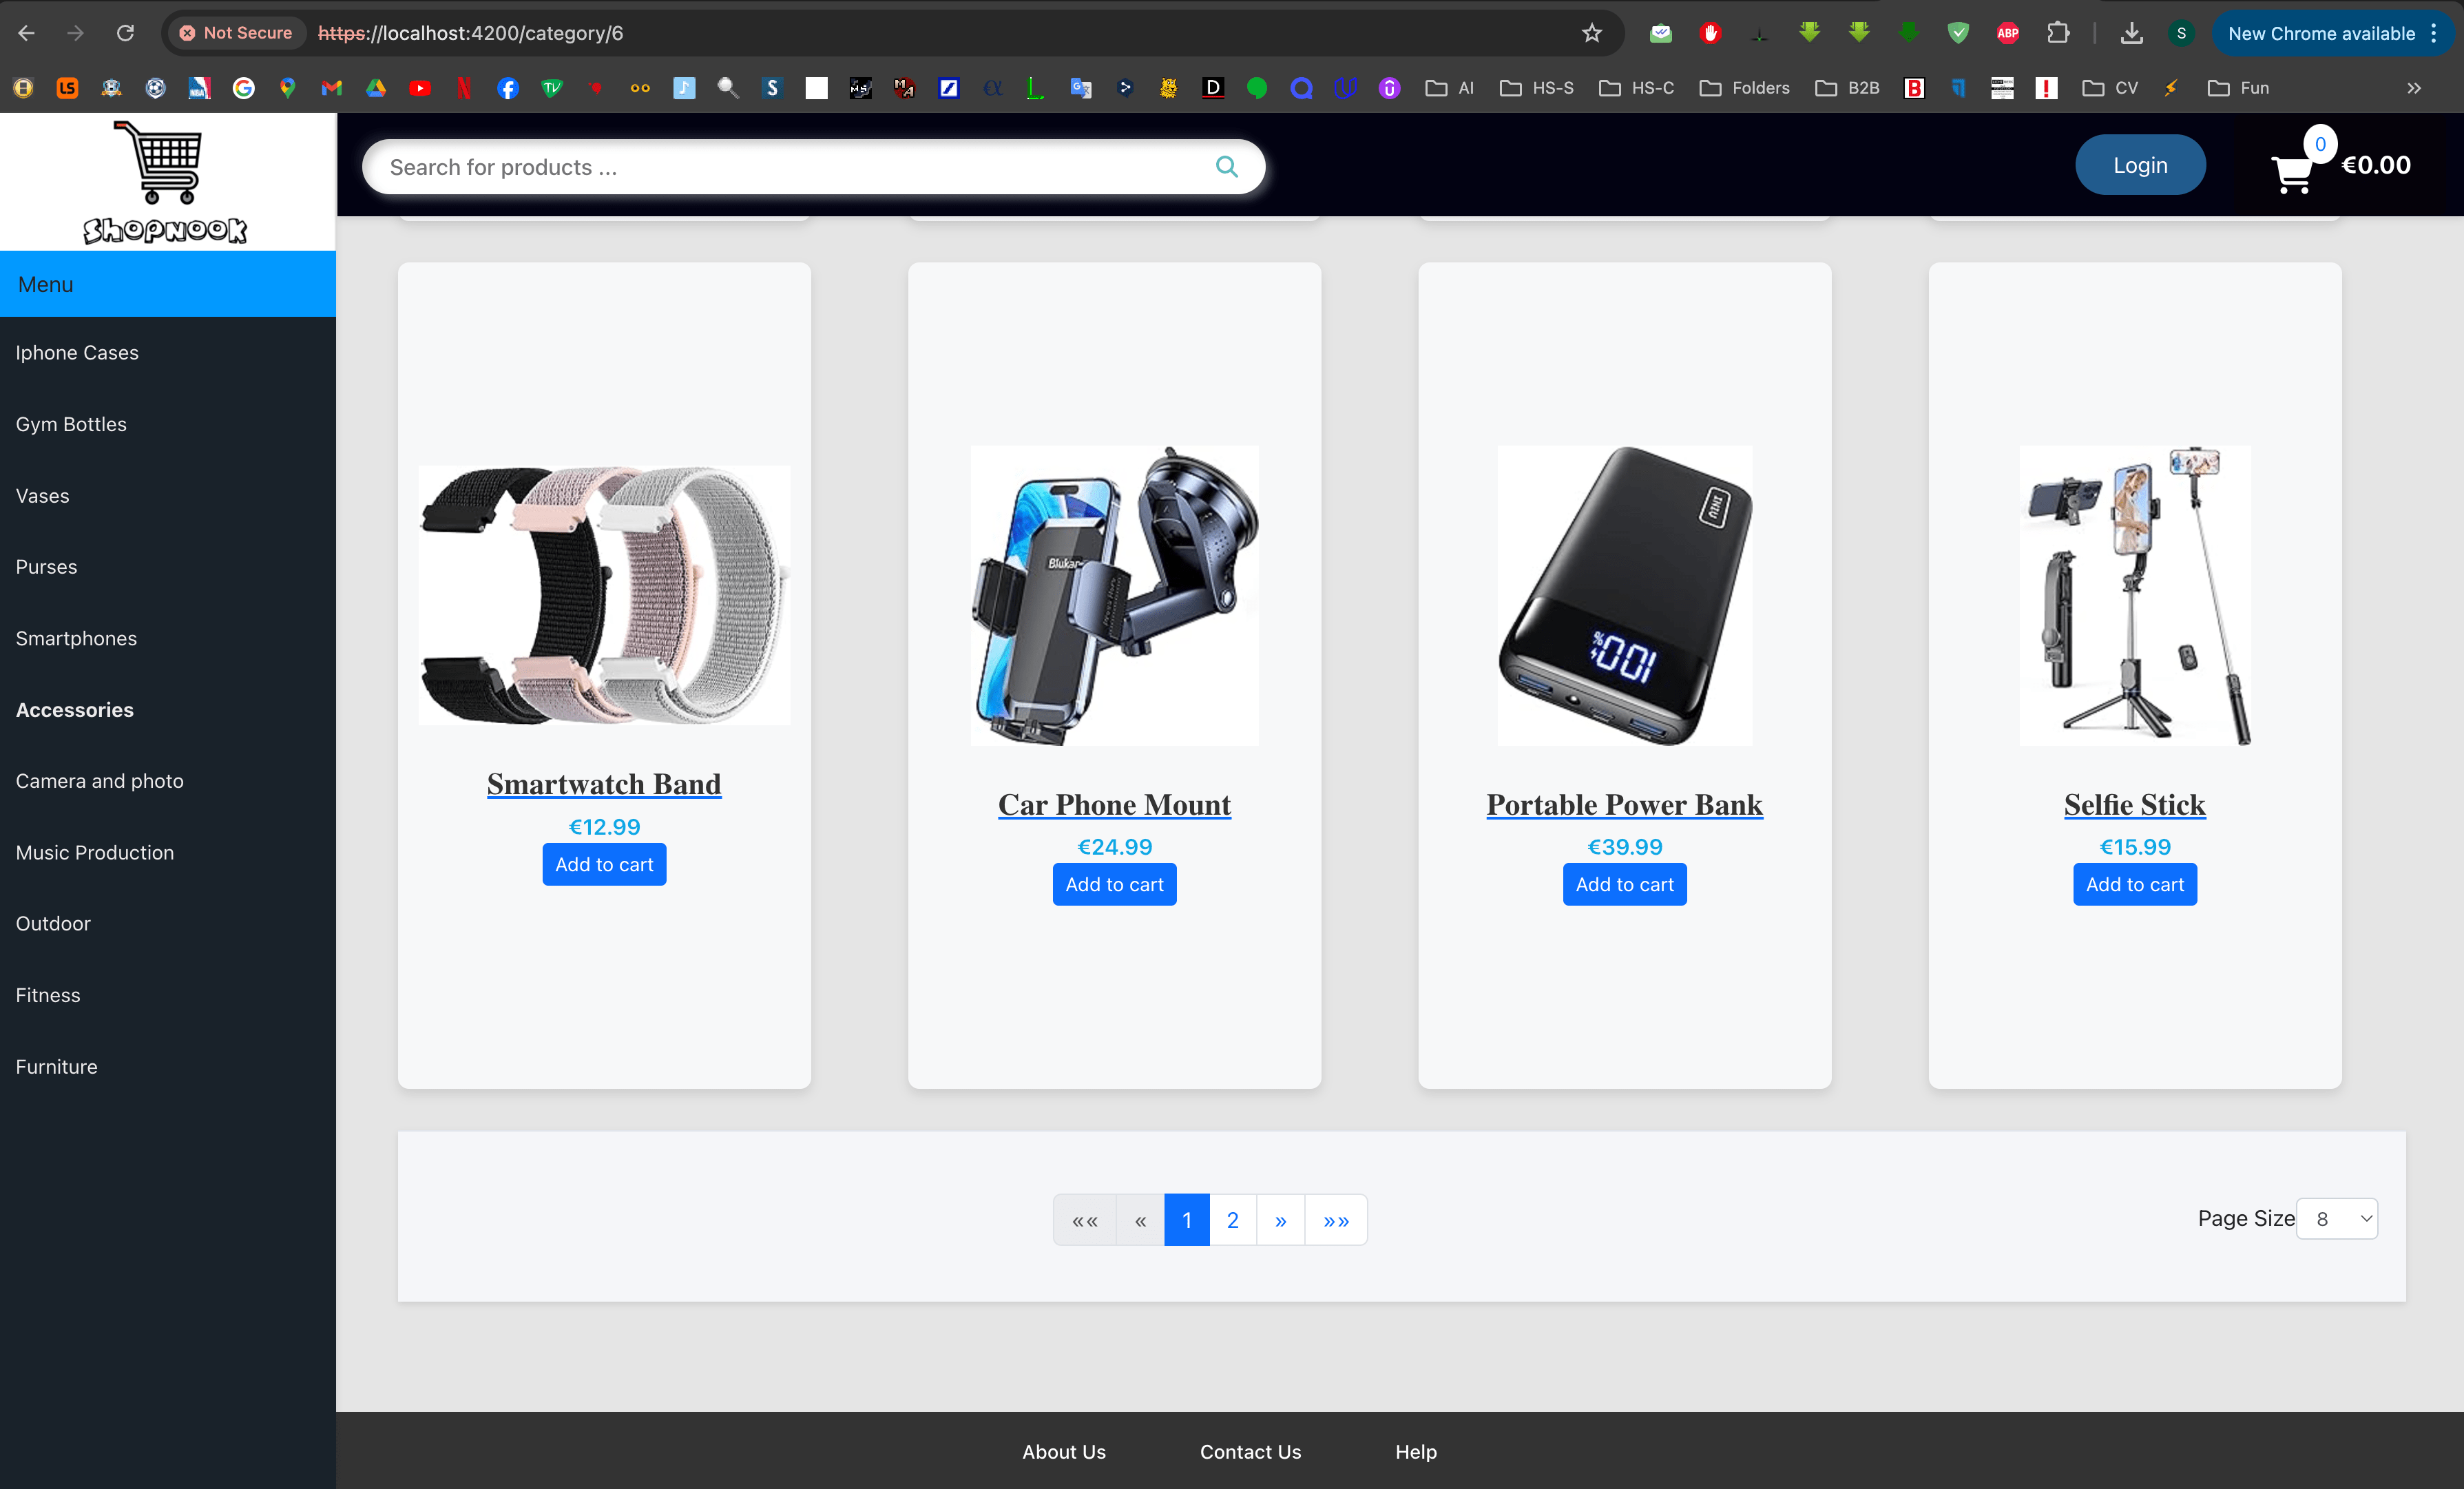
\includegraphics[width=0.9\textwidth]{Images/Home-Page.png} 
	\caption{Startseite} 
	\label{fig:sample-image} 
\end{figure}

 \subsection{Linke Seite}
 
Auf der linken Seite befindet sich:
\begin{itemize}
	\item \textbf{App-Logo:} Deutlich sichtbar auf der linken Seite, um eine gute Sichtbarkeit der Marke und eine einfache Navigation zurück zur Homepage zu gewährleisten.
	\item \textbf{Navigationsmenü:} Dieses Menü befindet sich unterhalb des Logos und bietet klare Produktkategorien, die das Surfen vereinfachen und einen schnellen Zugang zu den verschiedenen Produktbereichen ermöglichen.
\end{itemize}

 \subsection{Header}
 
In der Kopfzeile steht:
\begin{itemize}
	\item \textbf{Suchleiste:} Diese Suchleiste befindet sich am oberen Rand und ermöglicht es den Nutzern, Produkte durch die Eingabe von Schlüsselwörtern schnell zu finden, was die Effizienz der Produktsuche erhöht.
	\item \textbf{Anmeldeschaltfläche:} Diese Schaltfläche befindet sich in der Nähe der Suchleiste und bietet den Nutzern eine unkomplizierte Möglichkeit, sich in ihr Konto einzuloggen.
	\item \textbf{Warenkorb-Symbol:} Dieses Symbol befindet sich neben der Login-Schaltfläche und zeigt die Anzahl der Artikel im Warenkorb zusammen mit dem Gesamtpreis an, sodass die Nutzer einen schnellen Überblick über ihre Einkaufsaktivitäten erhalten.
\end{itemize}

 \subsection{Hauptinhalt}
Innerhalb des Hauptinhalts der Homepage gibt es:
\begin{itemize}
	\item \textbf{Produkt-Raster:} Zeigt Produkte in einem Rasterformat an, wobei jeder Eintrag gekennzeichnet ist:
	\begin{itemize}
		\item \textbf{Bild:} Bietet eine visuelle Vorschau des Produkts.
		\item \textbf{Preis:} Wird zur Transparenz deutlich angezeigt.
		\item \textbf{Titel:} Identifiziert das Produkt.
		\item \textbf{Link zu Details:} Führt den Nutzer zu einer Seite mit weiteren Informationen.
		\item \textbf{Schaltfläche „In den Warenkorb“:} Ermöglicht das schnelle Hinzufügen von Artikeln zum Einkaufswagen.
	\end{itemize}
	\item \textbf{Paginierung-Schaltflächen:} Diese Schaltflächen befinden sich am unteren Rand des Produkt-Rasters und ermöglichen es den Benutzern, durch mehrere Produktseiten zu navigieren.
\end{itemize}


 \subsection{Fußzeile}

Unten auf der Homepage gibt es Links zu
\begin{itemize}
	\item \textbf{About us:} Ein Link mit Informationen über Shopnook und sein Team.
	\item \textbf{Contact us:} Ein Link, über den Benutzer mit dem Kundendienst oder Support in Kontakt treten können.
	\item \textbf{Help:} Ein Link zu häufig gestellten Fragen oder Hilfsressourcen, die den Nutzern bei allgemeinen Fragen helfen.
\end{itemize}


\section{Warenkorb-Details}\index{Warenkorb-Details}

Die Abbildung zeigt eine typische Schnittstelle für einen Einkaufswagen.

\begin{figure}[H]  
	\centering % Centers the image
	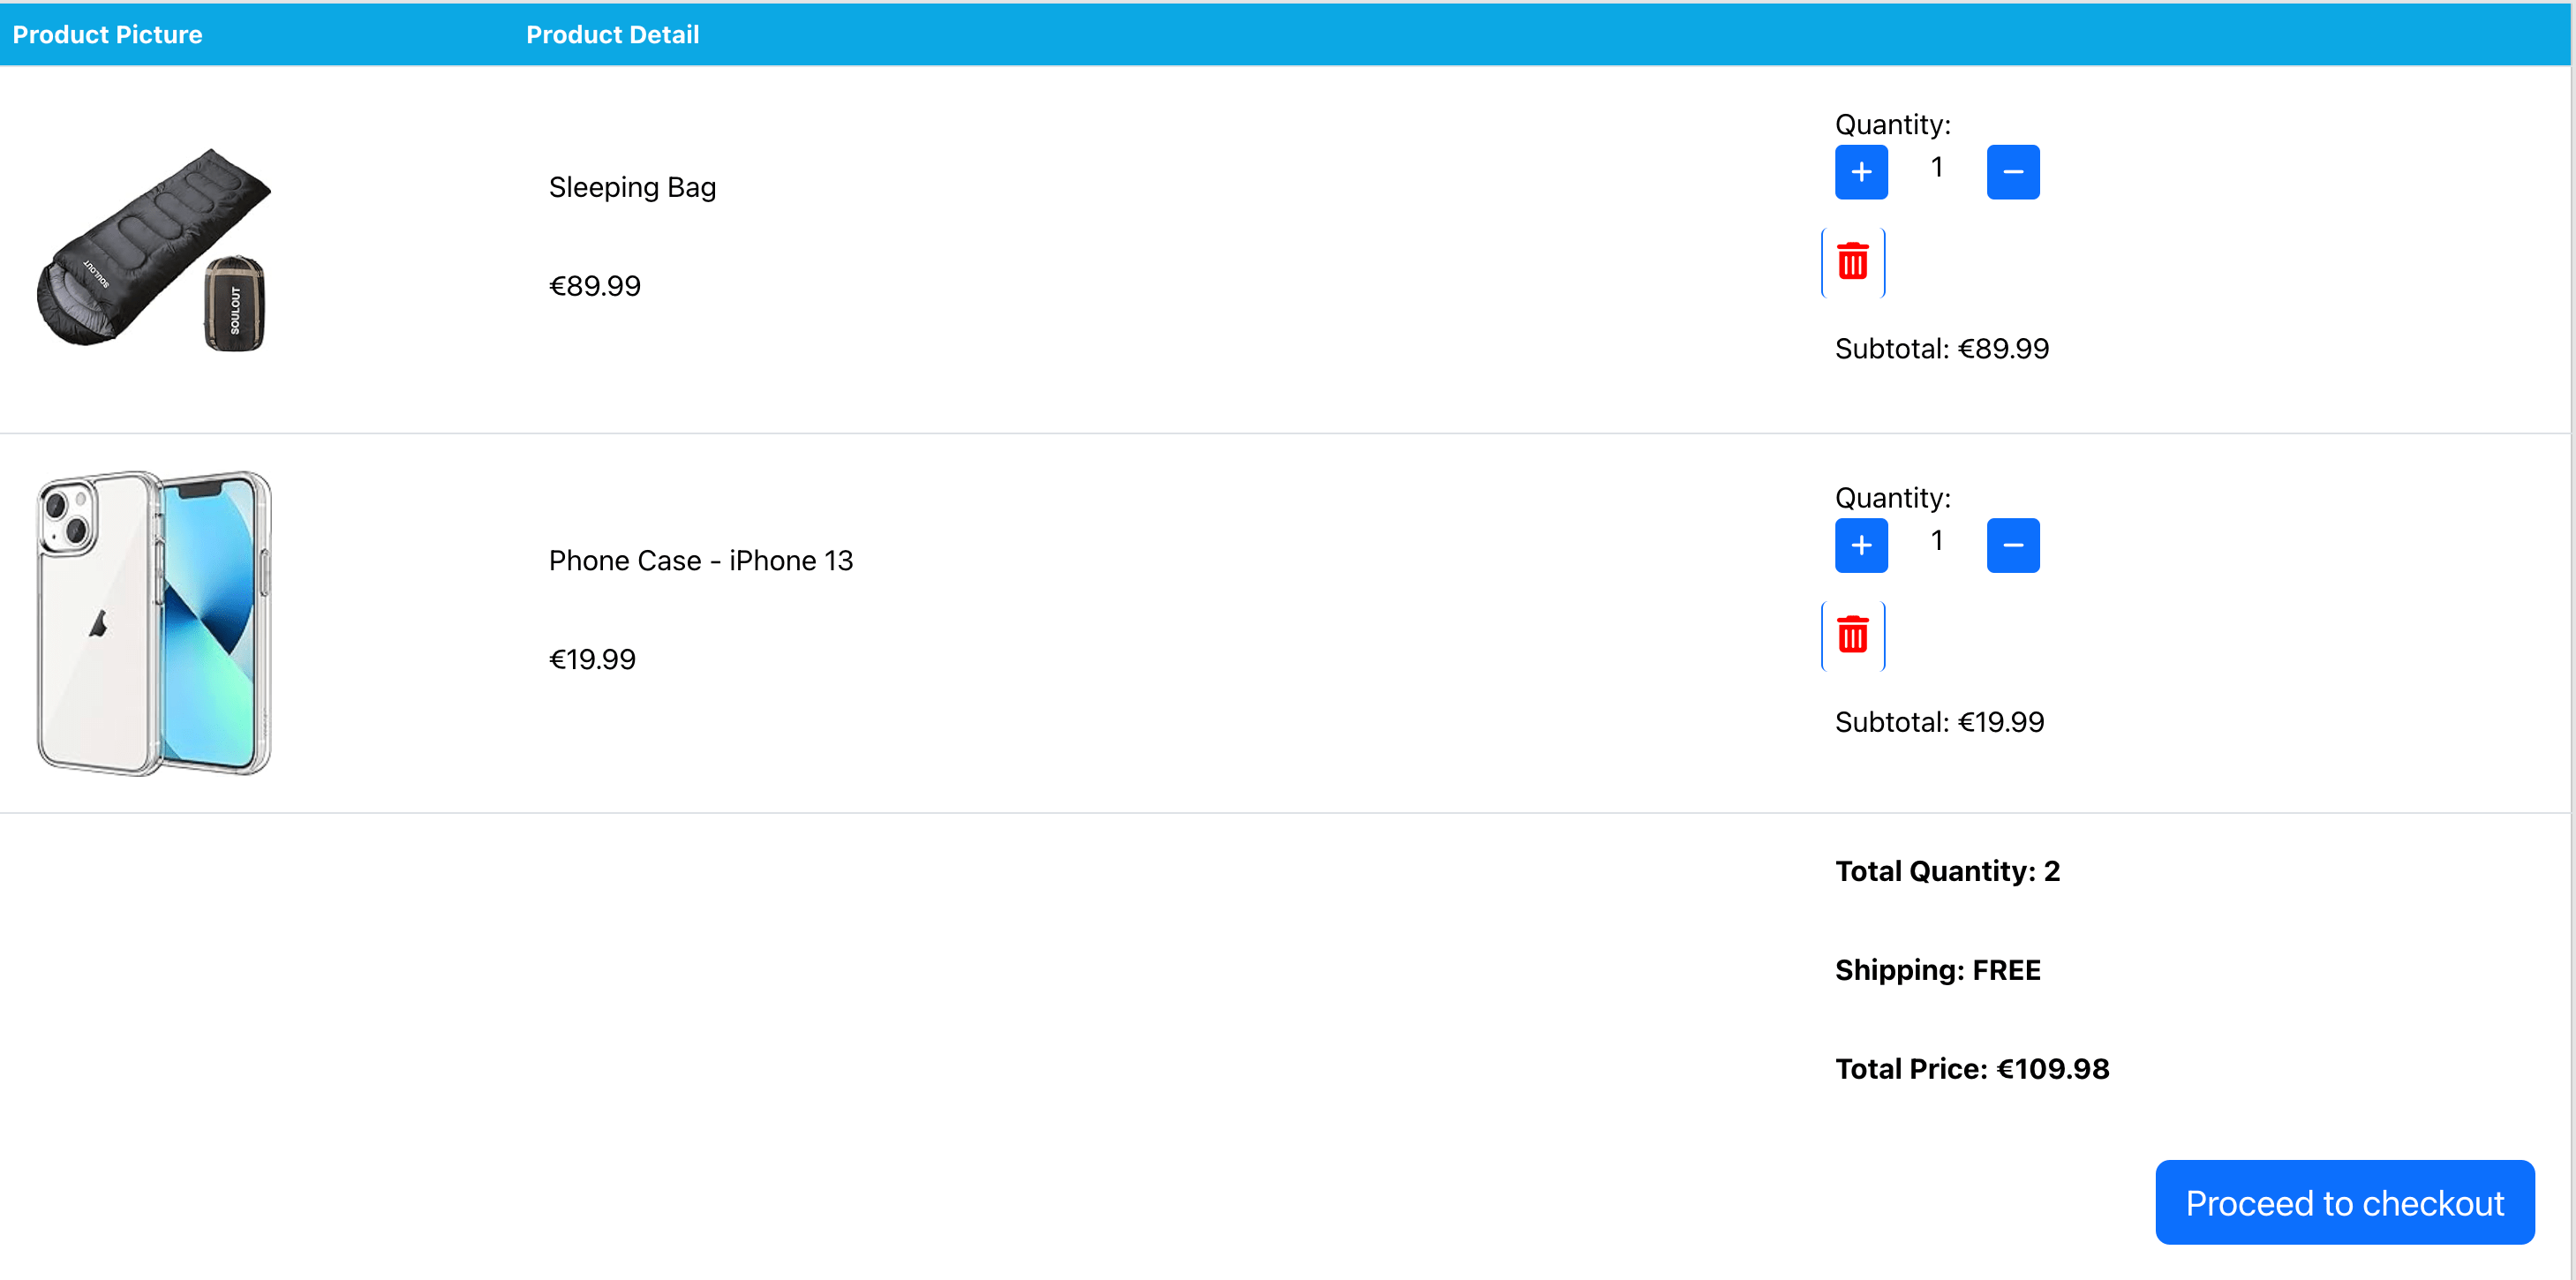
\includegraphics[width=0.9\textwidth]{Images/Cart-Details.png} 
	\caption{Warenkorb-Details} 
	\label{fig:sample2-image} 
\end{figure}

Die Detailseite des Warenkorbs bietet eine umfassende und benutzerfreundliche Schnittstelle, die mehrere Schlüsselelemente für ein optimales Einkaufserlebnis enthält. In der Produktliste werden alle Artikel angezeigt, die in den Warenkorb gelegt wurden, jeweils mit einem Bild und detaillierten Informationen. Der Benutzer kann seinen Warenkorb mit der Mengenkontrolle leicht verwalten, indem er die Menge jedes Produkts über Schaltflächen zum Erhöhen und Verringern anpasst oder Artikel nach Bedarf entfernt. Die Produktpreise werden übersichtlich dargestellt, einschließlich des Preises pro Einheit und der Zwischensummen, die auf der Grundlage der ausgewählten Menge berechnet werden. Die Bestellübersicht bietet einen Überblick über die Gesamtmenge der Artikel, wobei die Versandkosten als kostenlos gekennzeichnet sind und der endgültige Gesamtpreis deutlich angezeigt wird. Zur Erleichterung der nächsten Schritte im Kaufprozess ist eine auffällige Schaltfläche „Zur Kasse gehen“ enthalten, die den Benutzer zum Fortfahren mit der Bestellung anleitet.


\section{Checkout-Seite}\index{Checkout-Seite}
Nach einem Klick auf die Schaltfläche „Zur Kasse gehen“ leitet die Anwendung den Kunden zur Kassenseite weiter. Auf dieser Seite werden die Benutzer aufgefordert, ihre persönlichen Daten einzugeben, um den Kauf abzuschließen. Dazu gehören wichtige Angaben wie Name, Adresse und Zahlungsinformationen. Die Kassenseite ist so gestaltet, dass sie einen reibungslosen und sicheren Transaktionsprozess gewährleistet und den Benutzer durch die letzten Schritte zur Bestätigung seiner Bestellung und zum Abschluss des Kaufs führt.

Der erste Teil der Checkout-Seite (siehe unten) enthält ein Kundeninformationsformular, in dem die für die Auftragsabwicklung erforderlichen Angaben erfasst werden. Das Formular enthält Felder für grundlegende persönliche Informationen wie z. B.:

\begin{itemize}
	\item \textbf{Name:} Zur Identifizierung des Kunden.
	\item \textbf{Telefonnummer:} Für Kontaktzwecke.
	\item \textbf{E-Mail:} Für Auftragsbestätigungen und Aktualisierungen.
\end{itemize}

Darüber hinaus werden in dem Formular Informationen zur Lieferadresse erfasst:

\begin{itemize}
	\item \textbf{Land:} Zur Bestimmung der Versandregion.
	\item \textbf{Straße:} Die spezifische Lieferadresse.
	\item \textbf{Stadt:} Die Stadt für die genaue Zustellung.
	\item \textbf{Bundesland:} Das Bundesland oder die Provinz.
	\item \textbf{Postleitzahl:} Zur genauen Identifizierung des Standorts.
\end{itemize}

\begin{figure}[H]  
	\centering % Centers the image
	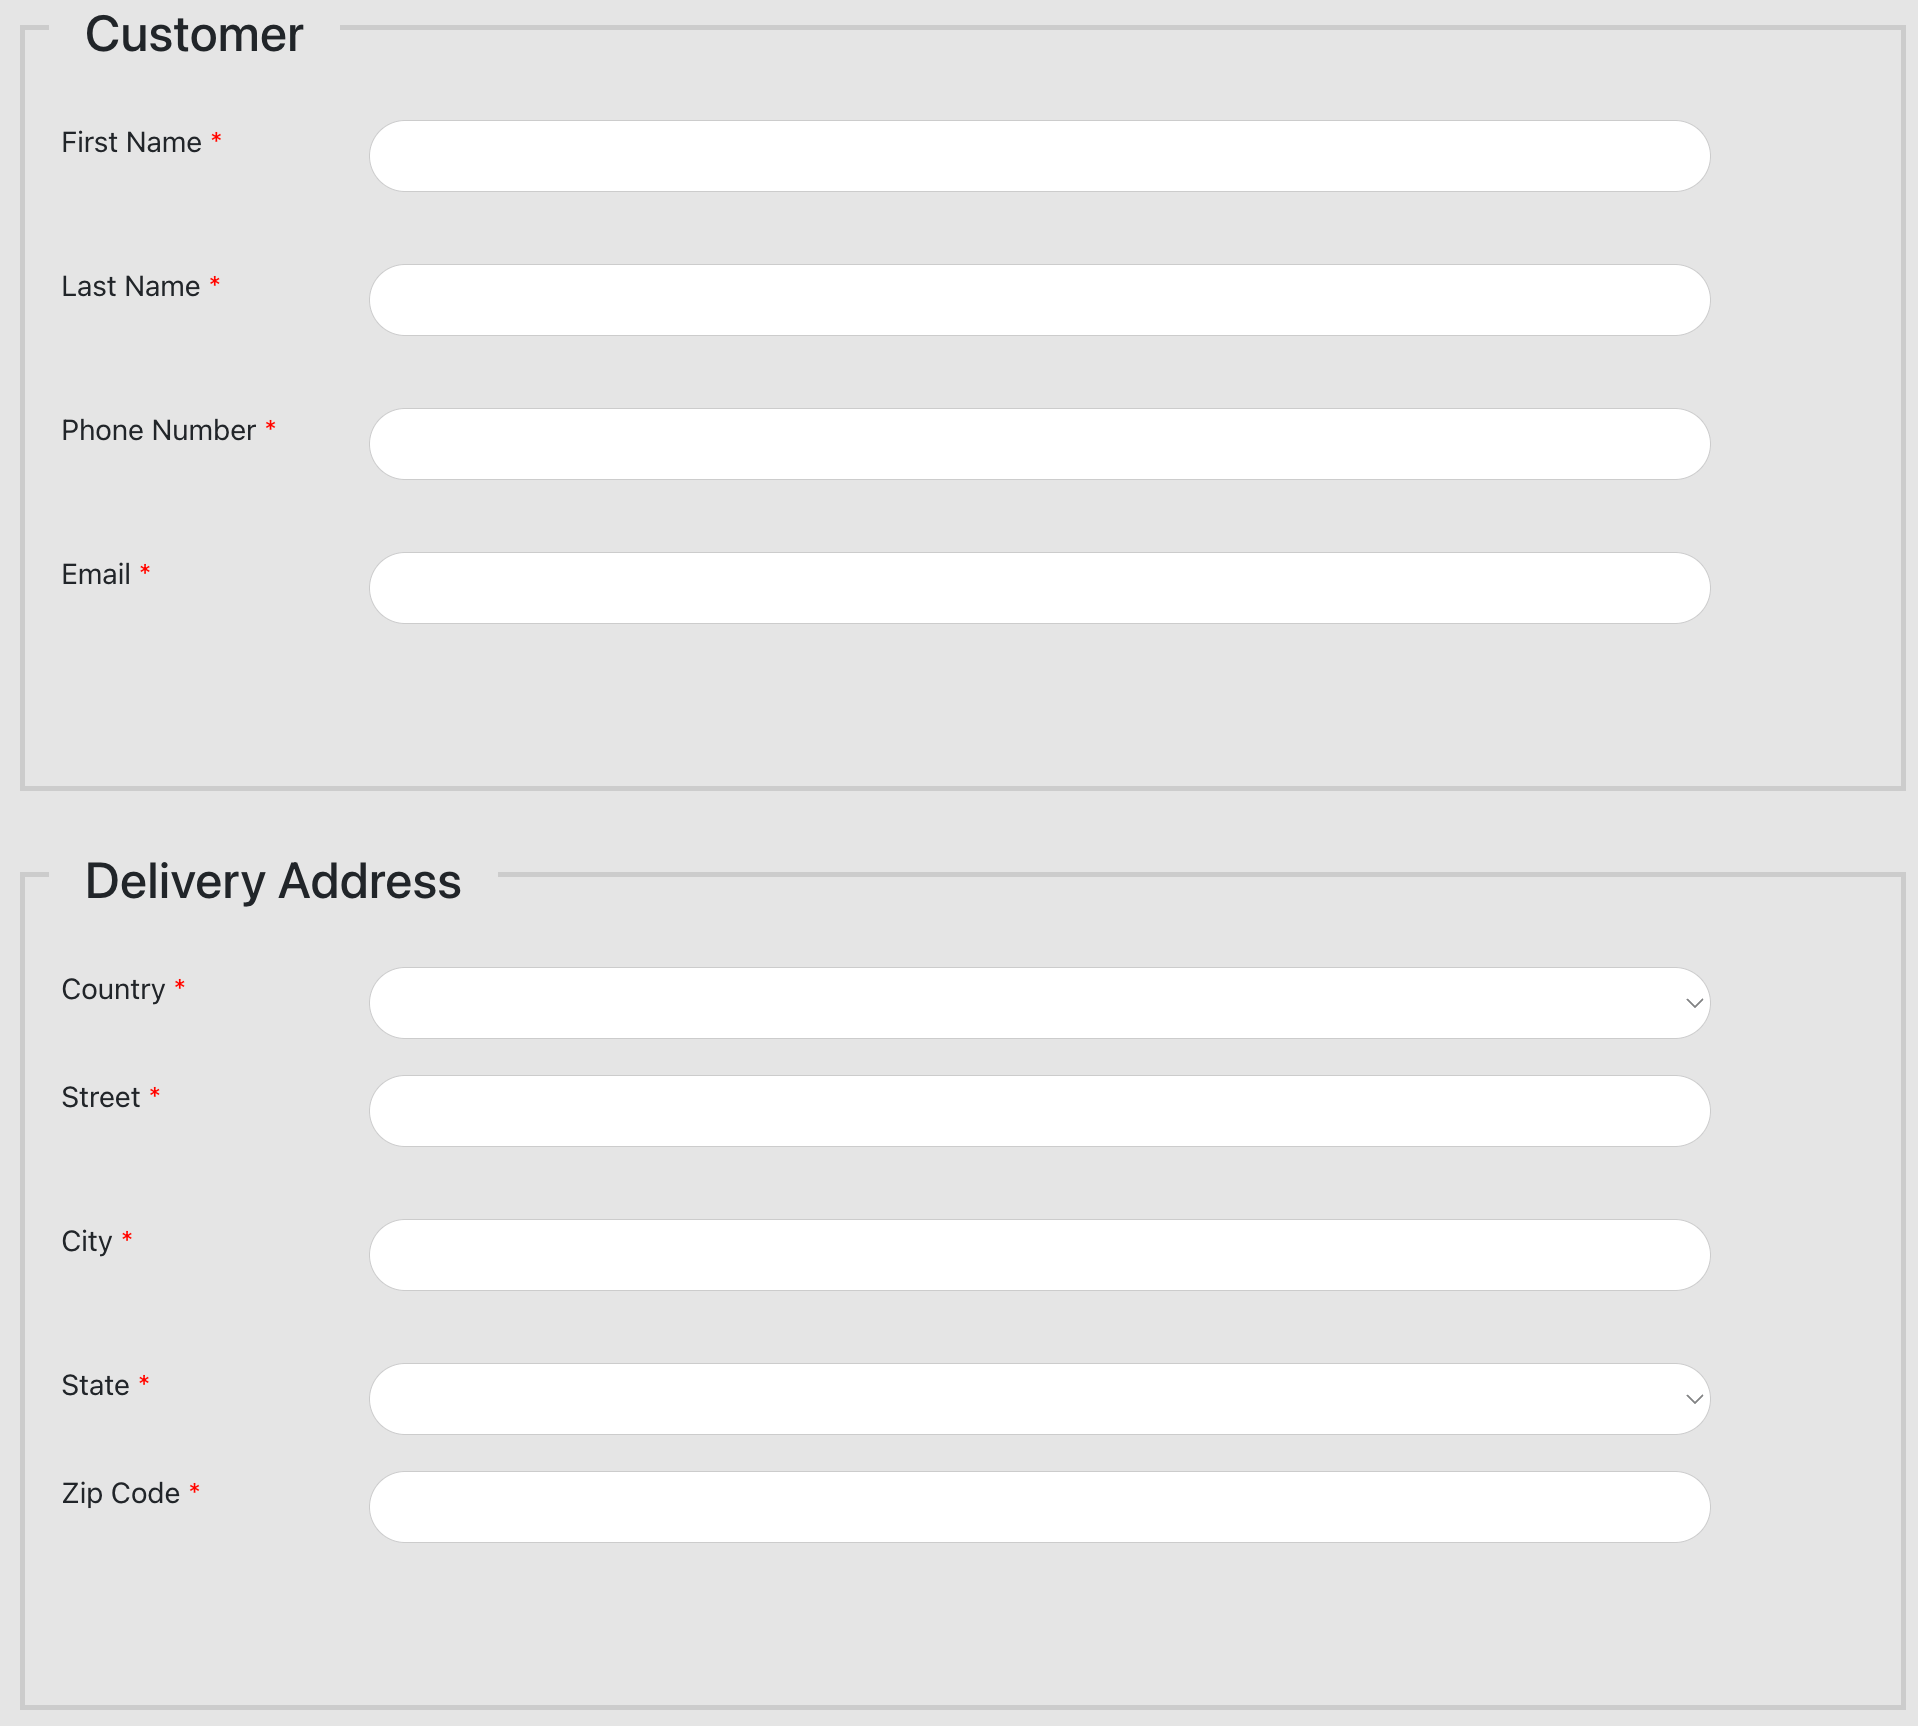
\includegraphics[width=0.9\textwidth]{Images/Checkout_1.png} 
	\caption{Checkout-1} 
	\label{fig:sample3-image} 
\end{figure}


















